\section{Технологическая часть}

\subsection{Средства реализации}

В таблице~\ref{tab:subd_comparison} представлено сравнение четырёх наиболее популярных реляционных систем управления базами данных (СУБД), таких как PostgreSQL, MySQL, Microsoft SQL Server и Oracle Database~\cite{DBEnginesRanking}. Для удобства использованы условные обозначения: <<+>> -- высокий уровень соответствия критерию, <<->> -- низкий уровень соответствия, <<+/->> -- частичное соответствие критерию с наличием определённых ограничений.

\begin{table}[h!]
	\centering
	\begin{tabular}{|p{5.2cm}|>{\centering\arraybackslash}p{3.0cm}|>{\centering\arraybackslash}p{2.0cm}|>{\centering\arraybackslash}p{2.3cm}|>{\centering\arraybackslash}p{2.3cm}|}
		\hline
		\textbf{Критерий} & \textbf{PostgreSQL} & \textbf{MySQL} & \textbf{MS SQL Server} & \textbf{Oracle} \\
		\hline
		Поддержка надёжности и ACID-свойств~\cite{Gray1981} & + & +/- & + & + \\
		\hline
		Совокупная стоимость владения & + & + & +/- & - \\
		\hline
	\end{tabular}
	\caption{Сравнительный анализ реляционных СУБД для информационной системы фитнес-клуба}
	\label{tab:subd_comparison}
\end{table}

В качестве СУБД выбрана \textbf{PostgreSQL}~\cite{postgresql}. Данная система поддерживает расширенные механизмы обеспечения целостности данных и предоставляет гибкие средства безопасности, включая разграничение доступа на уровне ролей и строк, что существенно повышает уровень защиты информации и позволяет реализовать строгие политики доступа. Особым преимуществом является то, что PostgreSQL распространяется по лицензии с открытым исходным кодом и не требует лицензионных платежей, что значительно снижает совокупную стоимость владения системой и делает её экономически выгодным решением для различных проектов. Кроме того, имеется практический опыт работы с этой системой, что снижает риски при внедрении.


Для кэширования данных используется  \textbf{Redis}~\cite{redis} -- является популярным решением~\cite{DBEnginesRanking}.

Для разработки интерфейса доступа выбран язык программирования \textbf{Swift}~\cite{swift}, так как он предоставляет все необходимые инструменты для эффективной работы с PostgreSQL и создания удобного пользовательского интерфейса. Кроме того, имеется практический опыт работы с этим языком.

В качестве средств разработки выбраны \textbf{Xcode}~\cite{xcode} и \textbf{pgAdmin 4}~\cite{pgadmin4}. Xcode обеспечивает полноценную среду для разработки интерфейсов на Swift, а pgAdmin 4 предоставляет все необходимые инструменты для управления базой данных PostgreSQL.

\subsection{Реализация базы данных}

Далее представлены реализации спроектированной базы данных: ее сущностей, ограничений целостности данных, ролевой модели и триггеров.

\subsubsection*{Реализация сущностей}

Реализации создания таблиц представлены на листингах~\ref{alg:1}-\ref{alg:12}.

\begin{lstlisting}[label=alg:1, caption=Реализация создания отношения Trainer, captionpos=t]
	CREATE TABLE "Trainer" (
	id 				UUID,
	user_id			UUID,
	description 	TEXT
	);
\end{lstlisting}

\begin{lstlisting}[label=alg:0, caption=Реализация создания отношения User, captionpos=t]
CREATE TABLE "User" (
	id 				UUID,
	email 			TEXT,
	phone_number 	TEXT,
	"password" 		TEXT,
	first_name 		TEXT,
	last_name 		TEXT,
	gender 			TEXT,
	birth_date 		DATE,
	"role"			TEXT
);
\end{lstlisting}

\begin{lstlisting}[label=alg:13, caption=Реализация создания отношения Specialization, captionpos=t]
CREATE TABLE "Specialization" (
	id	 	UUID,
	name 	TEXT
);
\end{lstlisting}

\newpage
\begin{lstlisting}[label=alg:4, caption=Реализация создания отношения TrainerSpecialization, captionpos=t]
CREATE TABLE "TrainerSpecialization" (
	id 					UUID,
	trainer_id			UUID,
	specialization_id	UUID,
	years				INT
);
\end{lstlisting}

\begin{lstlisting}[label=alg:5, caption=Реализация создания отношения MembershipType, captionpos=t]
CREATE TABLE "MembershipType" (
	id 			UUID,
	name 		TEXT,
	price 		NUMERIC,
	sessions	INT,
	days		INT
);
\end{lstlisting}

\begin{lstlisting}[label=alg:6, caption=Реализация создания отношения TrainingRoom, captionpos=t]
CREATE TABLE "TrainingRoom" (
	id			UUID,
	name	 	TEXT,
	capacity 	INT
);
\end{lstlisting}

\begin{lstlisting}[label=alg:9, caption=Реализация создания отношения Payment, captionpos=t]
CREATE TABLE "Payment" (
	id					UUID,
	user_id				UUID,
	membership_id		UUID,
	membership_type_id	UUID,
	transaction_id 		TEXT,
	"date" 				TIMESTAMP,
	"method" 			TEXT,
	gateway 			TEXT,
	status 				TEXT
);
\end{lstlisting}

\newpage
\begin{lstlisting}[label=alg:10, caption=Реализация создания отношенияMembership, captionpos=t]
CREATE TABLE "Membership" (
	id 					UUID,
	user_id				UUID,
	membership_type_id	UUID,
	start_date			DATE,
	end_date			DATE,
	available_sessions	INT
);
\end{lstlisting}

\begin{lstlisting}[label=alg:11, caption=Реализация создания отношения Training, captionpos=t]
CREATE TABLE "Training" (
	id 					UUID,
	specialization_id	UUID,
	room_id				UUID,
	trainer_id			UUID,
	"date"				TIMESTAMP
);
\end{lstlisting}

\begin{lstlisting}[label=alg:12, caption=Реализация создания отношения Attendance, captionpos=t]
	CREATE TABLE "Attendance" (
	id 				UUID,
	membership_id	UUID,
	training_id		UUID,
	status			TEXT
);
\end{lstlisting}


\subsubsection*{Реализация ограничений целостности данных}

Реализации ограничений целостности данных таблиц представлены на листингах~\ref{alg:17}-\ref{alg:26}.

\begin{lstlisting}[label=alg:17, caption=Реализация  ограничений целостности данных отношения Specialization, captionpos=t]
ALTER TABLE "Specialization"
	ADD CONSTRAINT "pk:specialization.id" PRIMARY KEY (id),
	ALTER COLUMN id SET DEFAULT gen_random_uuid(),
	ADD CONSTRAINT "chk:specialization.name:notnull" CHECK (
	name IS NOT NULL),
	ADD CONSTRAINT "chk:specialization.name:length" CHECK (
	length(name) < 128),
	ADD CONSTRAINT "uq:specialization.name" UNIQUE (name);
\end{lstlisting}

\newpage
\begin{lstlisting}[label=alg:14, caption=Реализация  ограничений целостности данных отношения User, captionpos=t]
ALTER TABLE "User"
	ADD CONSTRAINT "pk:user.id" PRIMARY KEY (id),
	ALTER COLUMN id SET DEFAULT gen_random_uuid(),
	ADD CONSTRAINT "chk:user.email:notnull" CHECK (email IS NOT NULL),
	ADD CONSTRAINT "chk:user.email:length" CHECK (length(email) < 128),
	ADD CONSTRAINT "chk:user.email:regexp" CHECK (
		email ~ '^[A-Za-z0-9._%-]+@[A-Za-z0-9.-]+[.][A-Za-z]+$'),
	ADD CONSTRAINT "uq:user.email" UNIQUE (email),
	ADD CONSTRAINT "chk:user.phone_number:notnull" CHECK (
		phone_number IS NOT NULL),
	ADD CONSTRAINT "chk:user.phone_number:length" CHECK (
		length(phone_number) < 32),
	ADD CONSTRAINT "chk:user.phone_number:regexp" CHECK (
		phone_number ~ '^\+\d{10,15}$'),
	ADD CONSTRAINT "uq:user.phone_number" UNIQUE (phone_number),
	ADD CONSTRAINT "chk:user.password:notnull" CHECK (
		"password" IS NOT NULL),
	ADD CONSTRAINT "chk:user.first_name:notnull" CHECK (
		first_name IS NOT NULL),
	ADD CONSTRAINT "chk:user.first_name:length" CHECK (
		length(first_name) < 128),
	ADD CONSTRAINT "chk:user.first_name:regexp" CHECK (
		first_name ~ '^([a-zA-Zа-яА-ЯёЁ]+(?:-[a-zA-Zа-яА-ЯёЁ]+)?)$'),
	ADD CONSTRAINT "chk:user.last_name:notnull" CHECK (
		last_name IS NOT NULL),
	ADD CONSTRAINT "chk:user.last_name:length" CHECK (
		length(last_name) < 128),
	ADD CONSTRAINT "chk:user.last_name:regexp" CHECK (
		last_name ~ '^([a-zA-Zа-яА-ЯёЁ]+(?:-[a-zA-Zа-яА-ЯёЁ]+)?)$'),
	ADD CONSTRAINT "chk:user.gender:notnull" CHECK (gender IS NOT NULL),
	ADD CONSTRAINT "chk:user.gender:length" CHECK (length(gender) < 32),
	ADD CONSTRAINT "chk:user.gender:regexp" CHECK (
		gender IN ('мужской', 'женский')),
	ADD CONSTRAINT "chk:user.birth_date:notnull" CHECK (
		birth_date IS NOT NULL),
	ADD CONSTRAINT "chk:user.birth_date" CHECK (
		birth_date BETWEEN 
			CURRENT_DATE - INTERVAL '120 years' AND 
			CURRENT_DATE - INTERVAL '14 years'
	ADD CONSTRAINT "chk:user.role:notnull" CHECK ("role" IS NOT NULL),
	ADD CONSTRAINT "chk:user.role:length" CHECK (length("role") < 32),
	ADD CONSTRAINT "chk:user.role:regexp" CHECK (
		"role" IN ('клиент', 'тренер', 'администратор')
	);
\end{lstlisting}

\begin{lstlisting}[label=alg:16, caption=Реализация  ограничений целостности данных отношения Trainer, captionpos=t]
ALTER TABLE "Trainer"
	ADD CONSTRAINT "pk:trainer.id" PRIMARY KEY (id),
	ALTER COLUMN id SET DEFAULT gen_random_uuid(),
	ADD CONSTRAINT "fk:trainer.user_id" FOREIGN KEY (user_id) 
		REFERENCES "User"(id) ON DELETE CASCADE,
	ADD CONSTRAINT "uq:trainer.user_id" UNIQUE (user_id),
	ALTER COLUMN "description" SET DEFAULT 'Нет описания.',
	ADD CONSTRAINT "chk:trainer.description:notnull" CHECK (
		description IS NOT NULL),
	ADD CONSTRAINT "chk:trainer.description:length" CHECK (
		length(description) < 512);
\end{lstlisting}

\begin{lstlisting}[label=alg:18, caption=Реализация  ограничений целостности данных отношения TrainerSpecialization, captionpos=t]
ALTER TABLE "TrainerSpecialization"
	ADD CONSTRAINT "pk:trainer_specialization.id" PRIMARY KEY (id),
	ALTER COLUMN id SET DEFAULT gen_random_uuid(),
	ADD CONSTRAINT "fk:trainer_specialization.trainer_id" 
		FOREIGN KEY (trainer_id) REFERENCES "Trainer"(id) ON DELETE CASCADE,
	ADD CONSTRAINT "fk:trainer_specialization.specialization_id" 
		FOREIGN KEY (specialization_id) 
		REFERENCES "Specialization"(id) ON DELETE CASCADE,
	ADD CONSTRAINT "uq:trainer_specialization.trainer+specialization" 
		UNIQUE (trainer_id, specialization_id),
	ALTER COLUMN years SET DEFAULT 0,
	ADD CONSTRAINT "chk:trainer_specialization.years:notnull" CHECK (
		years IS NOT NULL),
	ADD CONSTRAINT "chk:specialization.name:unsigned" CHECK (years >= 0);
\end{lstlisting}

\begin{lstlisting}[label=alg:25, caption=Реализация  ограничений целостности данных отношения Training, captionpos=t]
ALTER TABLE "Training"
	ADD CONSTRAINT "pk:training.id" PRIMARY KEY (id),
	ALTER COLUMN id SET DEFAULT gen_random_uuid(),
	ADD CONSTRAINT "fk:training.specialization_id" 
	FOREIGN KEY (specialization_id) 
	REFERENCES "Specialization"(id) ON DELETE SET NULL,
	ADD CONSTRAINT "fk:training.room_id" FOREIGN KEY (room_id) 
	REFERENCES "TrainingRoom"(id) ON DELETE SET NULL,
	ADD CONSTRAINT "fk:training.trainer_id" FOREIGN KEY (trainer_id) 
	REFERENCES "Trainer"(id) ON DELETE SET NULL,
	ALTER COLUMN "date" SET DEFAULT CURRENT_TIMESTAMP,
	ADD CONSTRAINT "chk:training.date:notnull" CHECK ("date" IS NOT NULL);
\end{lstlisting}

\newpage
\begin{lstlisting}[label=alg:23, caption=Реализация  ограничений целостности данных отношения Payment, captionpos=t]
ALTER TABLE "Payment"
	ADD CONSTRAINT "pk:payment.id" PRIMARY KEY (id),
	ALTER COLUMN id SET DEFAULT gen_random_uuid(),
	ADD CONSTRAINT "fk:payment.membership_id" FOREIGN KEY (membership_id) 
	REFERENCES "Membership"(id) ON DELETE SET NULL,
	ALTER COLUMN membership_id SET DEFAULT NULL,
	ADD CONSTRAINT "fk:payment.memshipt_id" FOREIGN KEY (membership_type_id) 
	REFERENCES "MembershipType"(id) ON DELETE SET NULL,
	ALTER COLUMN membership_type_id SET DEFAULT NULL,
	ADD CONSTRAINT "fk:payment.user_id" FOREIGN KEY (user_id) 
	REFERENCES "User"(id) ON DELETE SET NULL,
	ADD CONSTRAINT "chk:payment.user_id:notnull" CHECK (user_id IS NOT NULL),
	ADD CONSTRAINT "chk:payment.transaction_id:notnull" CHECK (
		transaction_id IS NOT NULL),
	ADD CONSTRAINT "chk:payment.transaction_id:length" CHECK (
		length(transaction_id) < 256),
	ADD CONSTRAINT "uq:payment.transaction_id" UNIQUE (transaction_id),
	ALTER COLUMN "date" SET DEFAULT CURRENT_TIMESTAMP,
	ADD CONSTRAINT "chk:payment.date:notnull" CHECK ("date" IS NOT NULL),
	ALTER COLUMN "method" SET DEFAULT 'наличные',
	ADD CONSTRAINT "chk:payment.method:notnull" CHECK ("method" IS NOT NULL),
	ADD CONSTRAINT "chk:payment.method:length" CHECK (length("method") < 64),
	ADD CONSTRAINT "chk:payment.method:regexp" CHECK (
		"method" IN ('наличные', 'кредитная карта', 'банковский перевод')),
	ALTER COLUMN "gateway" SET DEFAULT NULL,
	ADD CONSTRAINT "chk:payment.gateway:length" CHECK (
		length("gateway") < 64),
	ALTER COLUMN "status" SET DEFAULT 'ожидает',
	ADD CONSTRAINT "chk:payment.status:notnull" CHECK ("status" IS NOT NULL),
	ADD CONSTRAINT "chk:payment.status:length" CHECK (length("status") < 64),
	ADD CONSTRAINT "chk:payment.status" CHECK (
		status IN ('ожидает', 'оплачен', 'отменен'));
\end{lstlisting}

\begin{lstlisting}[label=alg:20, caption=Реализация  ограничений целостности данных отношения TrainingRoom, captionpos=t]
ALTER TABLE "TrainingRoom"
	ADD CONSTRAINT "pk:training_room.id" PRIMARY KEY (id),
	ALTER COLUMN id SET DEFAULT gen_random_uuid(),
	ADD CONSTRAINT "chk:training_room.name:notnull" CHECK (name IS NOT NULL),
	ADD CONSTRAINT "chk:training_room.name:length" CHECK (length(name) < 64),
	ADD CONSTRAINT "uq:training_room.name" UNIQUE (name),
	ADD CONSTRAINT "chk:training_room.capacity:notnull" CHECK (
	capacity IS NOT NULL),
	ADD CONSTRAINT "chk:training_room.capacity" CHECK (capacity > 0);
\end{lstlisting}

\begin{lstlisting}[label=alg:19, caption=Реализация  ограничений целостности данных отношения MembershipType, captionpos=t]
ALTER TABLE "MembershipType"
	ADD CONSTRAINT "pk:membership_type.id" PRIMARY KEY (id),
	ALTER COLUMN id SET DEFAULT gen_random_uuid(),
	ADD CONSTRAINT "chk:membership_type.name:notnull" CHECK (
	name IS NOT NULL),
	ADD CONSTRAINT "chk:membership_type.name:length" CHECK (
	length(name) < 128),
	ADD CONSTRAINT "uq:membership_type.name" UNIQUE (name),
	ALTER COLUMN price SET DEFAULT 0.0,
	ADD CONSTRAINT "chk:membership_type.price:notnull" CHECK (
	price IS NOT NULL),
	ADD CONSTRAINT "chk:membership_type.price:unsigned" CHECK (price >= 0.0),
	ALTER COLUMN sessions SET DEFAULT 1,
	ADD CONSTRAINT "chk:membership_type.sessions:notnull" CHECK (
	sessions IS NOT NULL),
	ADD CONSTRAINT "chk:membership_type.sessions:unsigned" CHECK (
	sessions > 0),
	ALTER COLUMN days SET DEFAULT 1,
	ADD CONSTRAINT "chk:membership_type.days:notnull" CHECK (
	days IS NOT NULL),
	ADD CONSTRAINT "chk:membership_type.days:unsigned" CHECK (days > 0);
\end{lstlisting}

\begin{lstlisting}[label=alg:24, caption=Реализация  ограничений целостности данных отношения Membership, captionpos=t]
ALTER TABLE "Membership"
	ADD CONSTRAINT "pk:membership.id" PRIMARY KEY (id),
	ALTER COLUMN id SET DEFAULT gen_random_uuid(),
	ADD CONSTRAINT "fk:membership.user_id" FOREIGN KEY (user_id) 
		REFERENCES "User"(id) ON DELETE CASCADE,
	ADD CONSTRAINT "fk:membership.membership_type_id" 
		FOREIGN KEY (membership_type_id) 
		REFERENCES "MembershipType"(id) ON DELETE SET NULL,
	ALTER COLUMN start_date SET DEFAULT NULL,
	ALTER COLUMN end_date SET DEFAULT NULL,
	ADD CONSTRAINT "chk:membership.dates:order" CHECK(
		(start_date IS NULL AND end_date IS NULL) OR (start_date IS NOT NULL 
		AND end_date IS NOT NULL AND start_date <= end_date)),
	ADD CONSTRAINT "uq:membership.membership_type+user"
		UNIQUE(membership_type_id, user_id),
	ALTER COLUMN available_sessions SET DEFAULT 0,
	ADD CONSTRAINT "chk:membership.available_sessions:notnull" CHECK (
		available_sessions IS NOT NULL),
	ADD CONSTRAINT "chk:membership.available_sessions:unsigned" CHECK (
		available_sessions >= 0);
\end{lstlisting}

\begin{lstlisting}[label=alg:26, caption=Реализация  ограничений целостности данных отношения Attendance, captionpos=t]
ALTER TABLE "Attendance"
	ADD CONSTRAINT "pk:attendance.id" PRIMARY KEY (id),
	ALTER COLUMN id SET DEFAULT gen_random_uuid(),
	ADD CONSTRAINT "fk:attendance.membership_id" FOREIGN KEY (membership_id) 
		REFERENCES "Membership"(id) ON DELETE CASCADE,
	ADD CONSTRAINT "fk:attendance.training_id" FOREIGN KEY (training_id) 
		REFERENCES "Training"(id) ON DELETE SET NULL,
	ADD CONSTRAINT "uq:attendance.membership+training" 
		UNIQUE (membership_id, training_id),
	ALTER COLUMN status SET DEFAULT 'ожидает',
	ADD CONSTRAINT "chk:attendance.status:notnull" CHECK (
		status IS NOT NULL),
	ADD CONSTRAINT "chk:attendance.status:length" CHECK (
		length(status) < 64),
	ADD CONSTRAINT "chk:attendance.status:regexp" CHECK (
		status IN ('посетил', 'отсутствовал', 'ожидает'));
\end{lstlisting}

\subsubsection{Реализация триггеров}

Реализации триггеров для автоматического обновления количества доступных занятий после посещения тренировки и записи на тренировку с учетом проверки количества доступных мест -- представлены на листингах~\ref{alg:27} и~\ref{alg:28} соответственно.

\begin{lstlisting}[label=alg:28, caption=Реализация триггера для записи на тренировку с учетом проверки количества доступных мест, captionpos=t]
CREATE OR REPLACE FUNCTION check_room_capacity()
RETURNS TRIGGER AS $$
BEGIN
	IF (TG_OP = 'INSERT') OR (TG_OP = 'UPDATE' AND NEW.training_id IS DISTINCT FROM OLD.training_id) 
	THEN
	IF (SELECT COUNT(*) FROM "Attendance" WHERE training_id = NEW.training_id) >= (SELECT capacity FROM "TrainingRoom" WHERE id = (SELECT room_id  FROM public.training WHERE id = NEW.training_id))
		THEN RAISE EXCEPTION 'Тренировка уже заполнена';
	END IF;
	END IF;
	RETURN NEW;
END; $$ LANGUAGE plpgsql;
CREATE OR REPLACE TRIGGER check_room_capacity_trigger
BEFORE INSERT ON "Attendance" FOR EACH ROW
EXECUTE FUNCTION check_room_capacity();
\end{lstlisting}

\begin{lstlisting}[label=alg:27, caption=Реализация триггера для автоматического обновления количества доступных занятий после посещения тренировки, captionpos=t]
CREATE OR REPLACE FUNCTION update_available_sessions()
RETURNS TRIGGER AS $$
BEGIN
	IF (NEW.status = 'посетил' OR NEW.status = 'отсутствовал') 
		AND (OLD.status <> 'посетил' AND OLD.status <> 'отсутствовал') 
	THEN
		UPDATE "Membership"
		SET available_sessions = available_sessions - 1
		WHERE id = NEW.membership_id;
	ELSIF (NEW.status = 'ожидает') 
		AND (OLD.status = 'посетил' OR OLD.status = 'отсутствовал') 
	THEN
		UPDATE "Membership"
		SET available_sessions = available_sessions + 1
		WHERE id = NEW.membership_id;
	END IF;
	RETURN NEW;
END; $$ LANGUAGE plpgsql;
CREATE OR REPLACE TRIGGER attendance_status_update
AFTER UPDATE OF status ON "Attendance"
FOR EACH ROW
EXECUTE FUNCTION update_available_sessions();
\end{lstlisting}

\subsubsection{Создание ролевой модели}

Реализация ролевой модели представлена на листингах~\ref{alg:30}, \ref{alg:31}, \ref{alg:32}, \ref{alg:33}, \ref{alg:34} и \ref{alg:35}.

\begin{lstlisting}[label=alg:30, caption=Реализация роли Guest (гость), captionpos=t]
CREATE ROLE guest WITH LOGIN;
GRANT EXECUTE ON FUNCTION register_user(
	UUID, TEXT, TEXT, TEXT, TEXT, TEXT, DATE, TEXT
) TO guest;
GRANT EXECUTE ON FUNCTION login_user(TEXT, TEXT) TO guest;
\end{lstlisting}

\begin{lstlisting}[label=alg:31, caption=Реализация роли Admin (администратор), captionpos=t]
CREATE ROLE admin WITH LOGIN PASSWORD 'admin' SUPERUSER BYPASSRLS;
GRANT ALL PRIVILEGES ON ALL TABLES IN SCHEMA public TO admin;
\end{lstlisting}

\begin{lstlisting}[label=alg:32, caption=Реализация ролей Client (клиент) и Trainer (тренер) -- начало, captionpos=t]
CREATE ROLE client WITH LOGIN PASSWORD 'client';
CREATE ROLE trainer WITH LOGIN PASSWORD 'trainer';
\end{lstlisting}

\begin{lstlisting}[label=alg:33, caption=Реализация ролей Client (клиент) и Trainer (тренер) -- продолжение, captionpos=t]
GRANT client TO trainer;
GRANT ALL ON "User" TO client;
GRANT ALL ON "User" TO trainer;
ALTER TABLE "User" ENABLE ROW LEVEL SECURITY;
CREATE POLICY personal_client_trainer_user_policy
	ON "User"
	FOR ALL
	TO client, trainer
	USING (id = current_user_id());
CREATE POLICY public_client_trainer_user_policy
	ON "User"
	FOR SELECT
	TO client, trainer
	USING (TRUE);
GRANT ALL ON "Trainer" TO client;
GRANT ALL ON "Trainer" TO trainer;
ALTER TABLE "Trainer" ENABLE ROW LEVEL SECURITY;
CREATE POLICY public_client_trainer_trainer_policy
	ON "Trainer"
	FOR SELECT
	TO client, trainer
	USING (TRUE);
CREATE POLICY personal_trainer_trainer_policy
	ON "Trainer"
	FOR ALL
	TO trainer
	USING (user_id = current_user_id());
GRANT ALL ON "Membership" TO client;
GRANT ALL ON "Membership" TO trainer;
ALTER TABLE "Membership" ENABLE ROW LEVEL SECURITY;
CREATE POLICY client_trainer_membership_policy
	ON "Membership"
	FOR ALL
	TO client, trainer
	USING (user_id = current_user_id());
CREATE POLICY trainer_membership_policy
	ON "Membership"
	FOR SELECT
	TO trainer
	USING (TRUE);
GRANT ALL ON "Payment" TO client;
GRANT ALL ON "Payment" TO trainer;
ALTER TABLE "Payment" ENABLE ROW LEVEL SECURITY;
\end{lstlisting}

\begin{lstlisting}[label=alg:34, caption=Реализация ролей Client (клиент) и Trainer (тренер) -- продолжение, captionpos=t]
CREATE POLICY client_trainer_payment_policy
	ON "Payment"
	FOR ALL
	TO client, trainer
	USING (user_id = current_user_id());
GRANT ALL ON "Attendance" TO client;
GRANT ALL ON "Attendance" TO trainer;
ALTER TABLE "Attendance" ENABLE ROW LEVEL SECURITY;
CREATE POLICY client_trainer_attendance_policy
	ON "Attendance"
	FOR ALL
	TO client, trainer
	USING (
		membership_id IN (
			SELECT id 
			FROM "Membership"
			WHERE user_id = current_user_id()
		)
	);
CREATE POLICY trainer_attendance_policy 
	ON "Attendance"
	FOR ALL
	TO trainer
	USING (
		training_id IN (
			SELECT id 
			FROM "Training"
			WHERE trainer_id = (
				SELECT id
				FROM "Trainer"
				WHERE user_id = current_user_id()
			)
		)
	);
GRANT SELECT ON "Specialization" TO client;
GRANT SELECT ON "Specialization" TO trainer;
GRANT SELECT ON "TrainerSpecialization" TO client;
GRANT SELECT ON "TrainerSpecialization" TO trainer;
GRANT ALL ON "Training" TO trainer;
GRANT ALL ON "Training" TO client;
ALTER TABLE "Training" ENABLE ROW LEVEL SECURITY;
CREATE POLICY client_training_select_policy
	ON "Training"
	FOR SELECT
\end{lstlisting}

\newpage
\begin{lstlisting}[label=alg:35, caption=Реализация ролей Client (клиент) и Trainer (тренер) -- конец, captionpos=t]
	TO client, trainer
	USING (TRUE);
CREATE POLICY trainer_training_update_policy
	ON "Training"
	FOR ALL
	TO trainer
	USING (
		trainer_id = (
			SELECT id 
			FROM "Trainer"
			WHERE user_id = current_user_id()
		)
	);
GRANT SELECT ON "MembershipType" TO client;
GRANT SELECT ON "MembershipType" TO trainer;
GRANT SELECT ON "TrainingRoom" TO client;
GRANT SELECT ON "TrainingRoom" TO trainer;
\end{lstlisting}

\subsection{Интерфейс для взаимодействая с базой данных}

Для взаимодействия с базой данных было разработано серверное программное обеспечение. Серверная часть предоставляет набор точек доступа по протоколу HTTP~\cite{HTTP_RFC7230} для выполнения операций создания, чтения, обновления и удаления данных. Все запросы обрабатываются в соответствии с принципами REST~\cite{Fielding2000} и документированы с использованием инструмента Swagger~\cite{Swagger}, что обеспечивает удобный доступ к спецификации прикладного программного интерфейса через веб-интерфейс (см. таблицу~\ref{tab:api-operations}).

На рисунках~\ref{fig:swagger_interface_1} и~\ref{fig:swagger_interface_2} показан интерфейс Swagger, который предоставляет визуализацию документации REST API и позволяет выполнять интерактивные запросы к сервису.

\begin{longtable}{|p{2cm}|p{7cm}|p{6cm}|}
	\hline
	\textbf{Метод} & \textbf{Путь} & \textbf{Описание} \\
	\hline
	\endfirsthead
	\hline
	\textbf{Метод} & \textbf{Путь} & \textbf{Описание} \\
	\hline
	\endhead
	\hline
	POST & /admin/attendances & Создать новое посещение \\
	\hline
	GET & /admin/attendances/all & Получить список всех посещений \\
	\hline
	DELETE & /admin/attendances/\{id\} & Удалить посещение по ID \\
	\hline
	PUT & /admin/attendances/\{id\} &  Обновить посещение по ID \\
	\hline
	\caption{Примеры операций интерфейса доступа}
	\label{tab:api-operations} 
\end{longtable}

\begin{figure}[ht!]
	\centering
	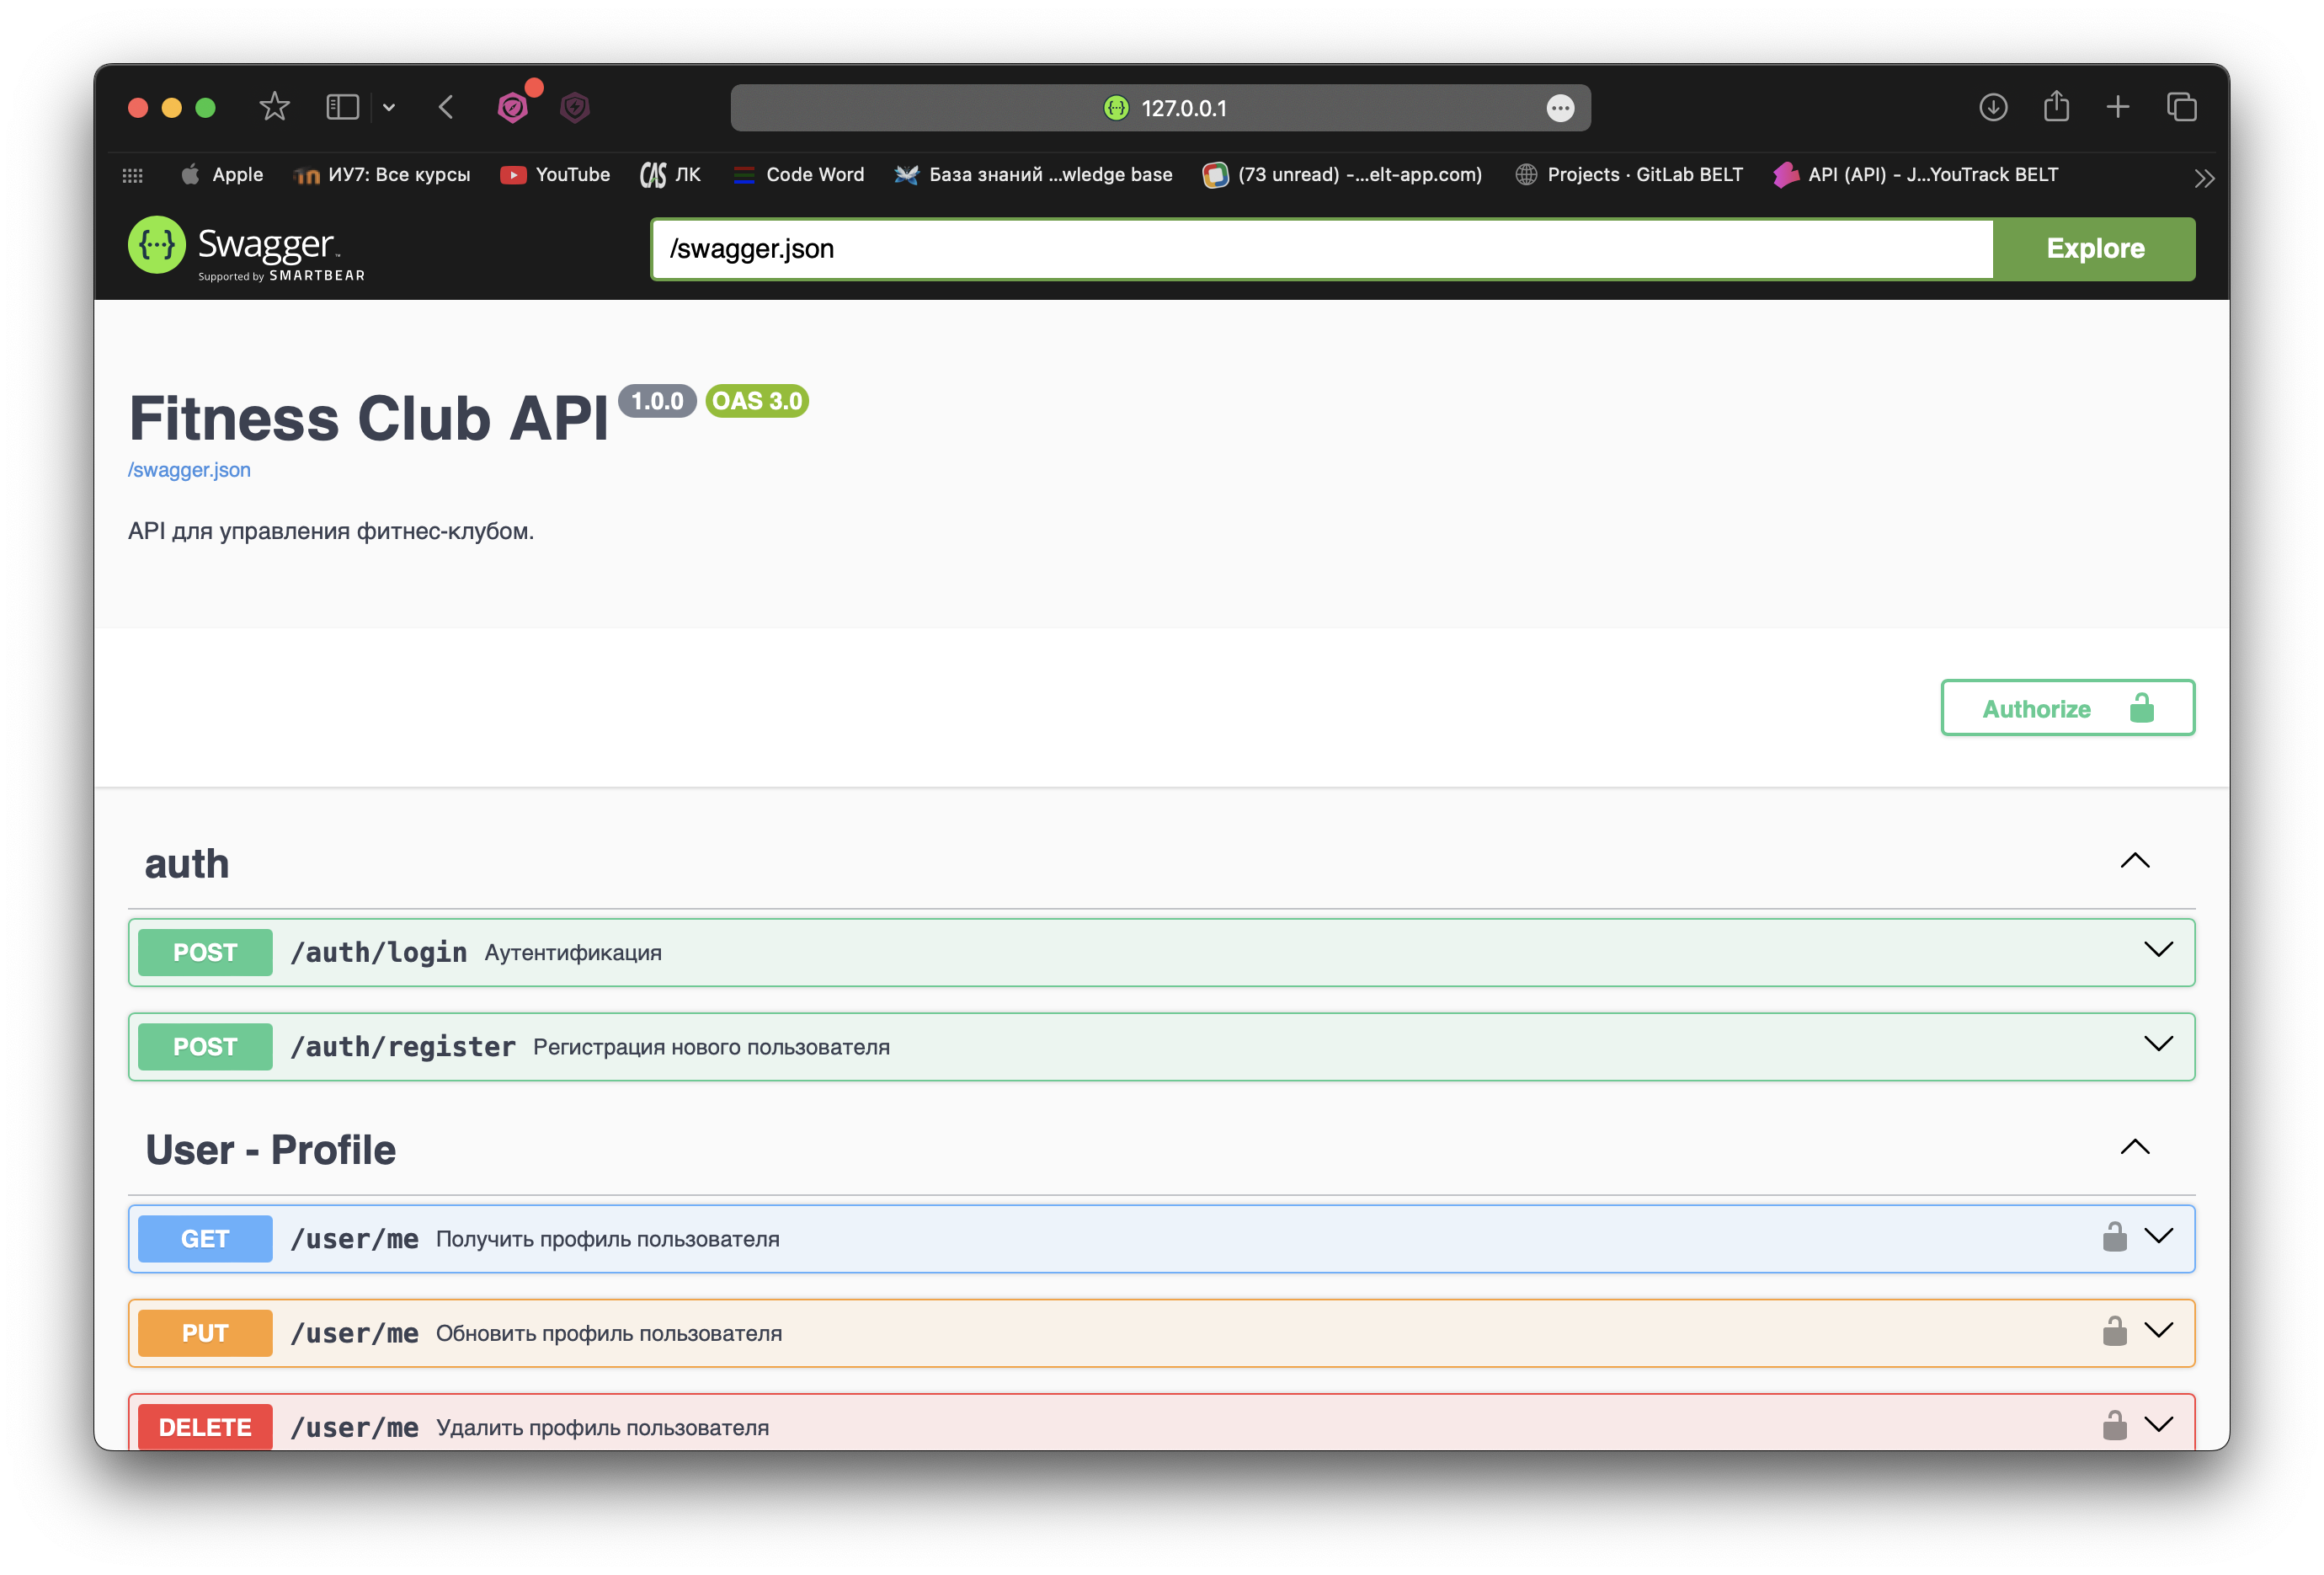
\includegraphics[scale=0.32]{./img/sw1.png}
	\caption{Главная страница интерфейса Swagger с перечнем доступных API}
	\label{fig:swagger_interface_1}
	
	\vspace{1em} % небольшой отступ между рисунками
	
	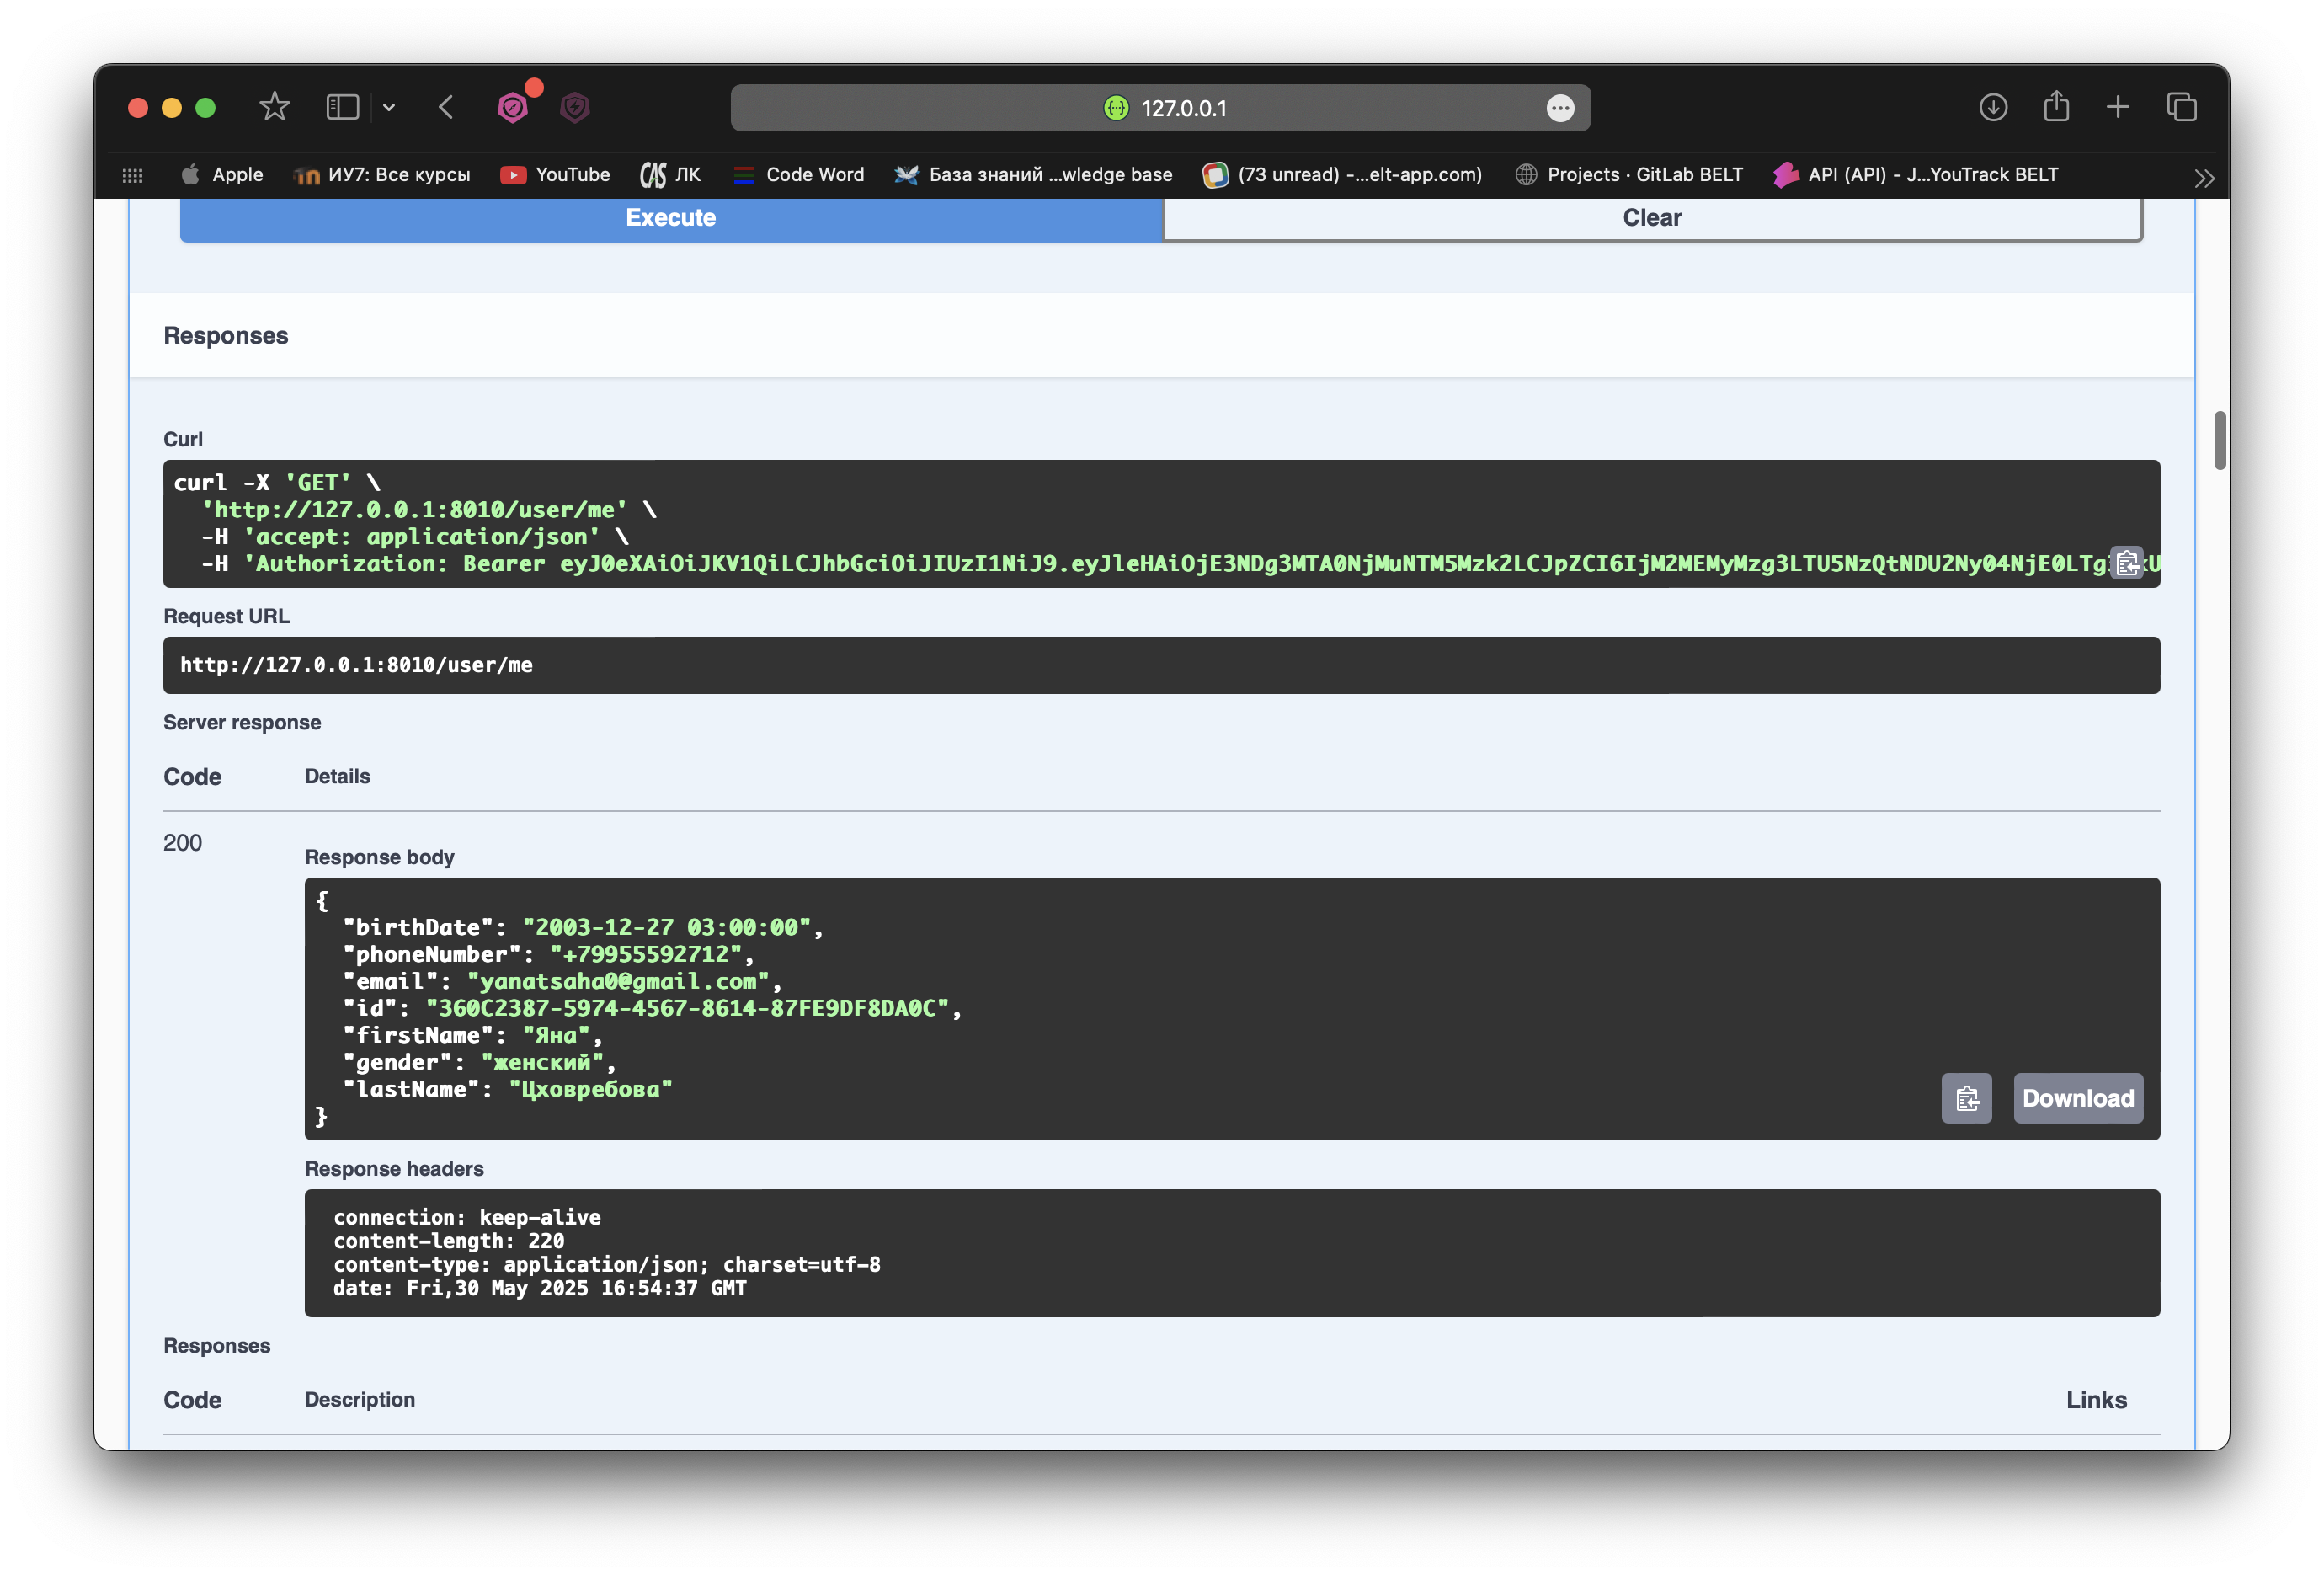
\includegraphics[scale=0.32]{./img/sw2.png}
	\caption{Пример запроса к эндпоинту \textit{GET /user/me} для получения данных авторизованного пользователя}
	\label{fig:swagger_interface_2}
\end{figure}


\subsection{Тестирование}

В таблицах~\ref{tab:trigger-tests-end} и~\ref{tab:trigger-tests-start} приведены результаты тестирования триггеров для автоматического обновления количества доступных занятий после посещения тренировки и для записи на тренировку с учётом проверки доступных мест.

\begin{table}[H]
	\centering
	\caption{Проверка корректности работы триггеров PostgreSQL -- начало}
	\label{tab:trigger-tests-end}
	\begin{tabular}{|c|p{5.5cm}|p{5cm}|p{4cm}|}
		\hline
		\textbf{№} & \textbf{Входные данные} & \textbf{Ожидаемый \newline результат} & \textbf{Фактический результат} \\
		\hline
		
		\multicolumn{4}{|c|}{\textbf{Триггер update\_available\_sessions}} \\
		\hline
		
		6 & Статус \textit{Attendance} меняется с <<ожидает>> на <<посетил>> & Значение \textit{available\_sessions} уменьшается на 1 & Уменьшено на 1 \\
		\hline
		
		7 & Статус \textit{Attendance} меняется с <<ожидает>> на <<отсутствовал>> & Значение \textit{available\_sessions} уменьшается на 1 & Уменьшено на 1 \\
		\hline
		
		8 & Статус  \textit{Attendance} меняется с <<посетил>> на <<ожидает>> & Значение \textit{available\_sessions} увеличивается на 1 & Увеличено на 1 \\
		\hline
		
		9 & Статус\textit{Attendance}  меняется с <<отсутствовал>> на <<ожидает>> & Значение \textit{available\_sessions} увеличивается на 1 & Увеличено на 1 \\
		\hline
		
		10 & Статус\textit{Attendance}  меняется с <<посетил>> на <<посетил>> & \textit{available\_sessions} не изменяется & Значение не изменилось \\
		\hline
		
		11 & Статус \textit{Attendance} меняется с <<ожидает>> на <<ожидает>> & \textit{available\_sessions} не изменяется & Значение не изменилось \\
		\hline
		
		12 & Запись \textit{Attendance} изменяется, но статус не трогается & \textit{available\_sessions} не изменяется & Значение не изменилось \\
		\hline
	\end{tabular}
\end{table}


\begin{table}[H]
	\centering
	\caption{Проверка корректности работы триггеров PostgreSQL -- конец}
	\label{tab:trigger-tests-start}
 	\begin{tabular}{|c|p{5.5cm}|p{5cm}|p{4cm}|}
		\hline
		\textbf{№} & \textbf{Входные данные} & \textbf{Ожидаемый \newline результат} & \textbf{Фактический результат} \\
		\hline
		
		\multicolumn{4}{|c|}{\textbf{Триггер check\_room\_capacity}} \\
		\hline
		
		1 & Вставка новой записи в \textit{Attendance}, \textit{training\_id} указывает на тренировку с незаполненной комнатой & Запись добавляется успешно & Запись добавлена \\
		\hline
		
		2 & Вставка новой записи в \textit{Attendance}, когда количество уже достигло \textit{capacity} в \textit{TrainingRoom} & Ошибка: \textit{Тренировка уже заполнена} & Ошибка выдана \\
		\hline
	\end{tabular}
\end{table}

\subsection*{Вывод}

В данном разделе представлены выбранные средства реализации, приведены реализации сущностей, ограничений целостности данных, ролевой модели и триггеров. Также описано тестирование триггеров и описан интерфейс, обеспечивающий взаимодействие с базой данных.